\newpage
\section{Construction}
\subsection{Database schema}
\hspace{0.7cm}The database is the information source that our whole project bases on. Here, we designed our database to have 4 fundamental tables that every restaurant management system should have, and all of these 4 tables relates to each other:

\vspace{2cm}
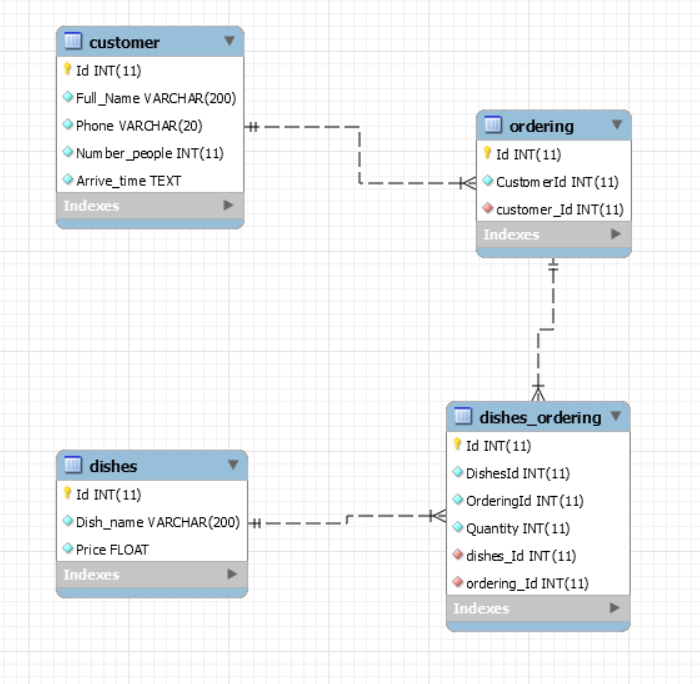
\includegraphics{images/database schema.png}

\newpage
\vspace{6cm}
\subsubsection{Relationship between tables}
\begin{itemize}
  \item Customer – Ordering: one to many relationship (One customer can have many orders but one order can belong to an exact customer) 
  \item Dishes – Ordering: many to many relationship (One dish can belong to many orders and vice versa) 
\end{itemize}

\vspace{0.5cm}
\subsubsection{Tables’ functions}
\begin{itemize}
  \item Customer: key information of a customer.
  \item Dishes: data of all dishes in the menu. 
  \item Ordering: contains customers’ ID implementing which order belongs to which customer.
  \item Dishes\_Ordering: intermediary table between dishes and ordering table which contains the quantity of each dish ordered.
\end{itemize}

\newpage
\subsection{Python modules, classes and packages}
\hspace{0.7cm}Since the amount of code is quite large, we decided so split the whole project into small parts in order to handle everything easily:

\vspace{1cm}
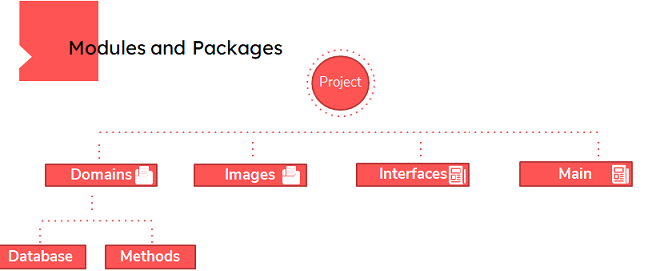
\includegraphics{images/modules and package.png}
\hspace{0.7cm}Firstly, we divided the code into 2 packages: \textbf{“Domains”, “Images”} and 2 modules \textbf{“Interfaces”, “Main”}

\begin{enumerate}
  \item \textbf{"Domain"} package: contains everything related to the database
    \begin{itemize}
        \item \textbf{"restaurant.SQL"} file: the database of the restaurant in SQL file
        \item \textbf{"SQL.py"}: a Python module that deals with the database. It has 2 classes: 
            \begin{itemize}
                \item \textbf{class sqll} is responsible for the CRUD methods;
                \item \textbf{class buttons} connects the database to the interface. To be more specific, we took advantage of “mysql.connector” module in “mysql-connector-python” package to link them together 
            \end{itemize}
    \end{itemize}
  \item \textbf{"Images"} package: has the images that we use in our interface
  \item \textbf{"INTERFACE.py"}: a Python module that created the layout of the user interface by \textit{“tkinter”} toolkit. It has only 1 class named \textbf{“class interface”}
  \item \textbf{"main.py"}: another Python module that is able to run the program
\end{enumerate}